\documentclass{report}
\setlength{\parskip}{0pt} % esp. entre parrafos
\setlength{\parindent}{20pt} % esp. al inicio de un parrafo
\usepackage{amsmath} % mates
\usepackage{listings}
\usepackage{xcolor}
\usepackage[sort&compress,numbers]{natbib} % referencias
\usepackage{url} % que las URLs se vean lindas
\usepackage[top=10mm,left=20mm,right=20mm,bottom=25mm]{geometry} % \textbf{\textbf{}}margenes
\usepackage{hyperref} % ligas de URLs
\usepackage{graphicx} % poner figuras
\usepackage{caption}
\usepackage{subcaption}
\usepackage[spanish]{babel} % otros idiomas
\hypersetup{
    colorlinks=true,
    linkcolor=blue,
    filecolor=blue,      
    urlcolor=blue,
}
\renewcommand{\lstlistingname}{C\'odigo}
\definecolor{codegreen}{rgb}{0,0.6,0}
\definecolor{codegray}{rgb}{0.5,0.5,0.5}
\definecolor{codepurple}{rgb}{0.58,0,0.82}
\definecolor{backcolour}{rgb}{0.95,0.95,0.92}
\lstdefinestyle{mystyle}{
    backgroundcolor=\color{backcolour},   
    commentstyle=\color{codegreen},
    keywordstyle=\color{magenta},
    numberstyle=\tiny\color{codegray},
    stringstyle=\color{codepurple},
    basicstyle=\ttfamily\footnotesize,
    breakatwhitespace=false,         
    breaklines=true,                 
    keepspaces=true,                 
    numbers=left,                    
    numbersep=5pt,                  
    showspaces=false,                
    showstringspaces=false,
    showtabs=false,                  
    tabsize=2
}
\lstset{style=mystyle}

\title{Reporte 9:\\Interacciones entre Part\'iculas}
\author{Jorge Torres}
\date{\today}

\begin{document}

\maketitle

\chapter{Part\'iculas con Carga y con Masa}

\section{Objetivo}
En esta pr\'actica se trabaja con un modelo simplificado de los fen\'omenos de atracci\'on y repulsi\'on de cargas el\'ectricas, adem\'as del fen\'omeno de atracci\'on gravitacional. El modelo consiste en una cantidad $n$ de part\'iculas que cuentan con una carga el\'ectrica, las cargas del mismo signo se repelen, mientras que las de signo opuesto se atraen. Adem\'as, cada part\'icula cuenta con una masa, lo que genera una fuerza de atracci\'on gravitacional entre ellas. El objetivo es estudiar la distribución de velocidades de las partículas y verificar gráficamente que esté presente una relación entre los tres factores: la velocidad, la magnitud de la carga, y la masa de las partículas.

\section{Desarrollo}
El desarrollo est\'a basado en el \href{https://github.com/satuelisa/Simulation/blob/master/Particles/interaction.py}{c\'odigo} implementado por E. Schaeffer para simular las part\'iculas \'unicamente con carga el\'ectrica \cite{elisa1}. Con el c\'odigo \ref{codigo1} se crean 25 part\'iculas, normal y aleatoriamente distribu\'idas con coordenadas $(x, y)$ en un plano, adem\'as se les asigna una carga $c$ y una masa $m$ distribu\'idas de la misma manera. Los c\'odigos completos se pueden encontrar en el repositorio en GitHub de J. Torres \cite{jorge1}.

\begin{lstlisting}[caption=Creaci\'on de Part\'iculas, label=codigo1, language=Python]
n = 25
x = np.random.normal(size = n)
y = np.random.normal(size = n)
c = np.random.normal(size = n)
m = np.random.normal(size = n)
\end{lstlisting}

El c\'odigo \ref{codigo2} asegura que las posiciones de las part\'iculas oscilen entre 0 y 1, que sus cargas oscilen entre -1 y 1, y que sus masas sean n\'umeros enteros entre 0 y 10, exceptuando masas nulas.

\begin{lstlisting}[caption={Distribuci\'on de Part\'iculas, Cargas y Masas}, label=codigo2, language=Python]
xmax = max(x)
xmin = min(x)
x = (x - xmin) / (xmax - xmin)
ymax = max(y)
ymin = min(y)
y = (y - ymin) / (ymax - ymin) 
cmax = max(c)
cmin = min(c)
c = 2 * (c - cmin) / (cmax - cmin) - 1
mmax = max(m)
mmin = min(m)
m = 10 * ((m - mmin) / (mmax - mmin) + 0.1)
m = np.round(m).astype(int)
\end{lstlisting}

Con el c\'odigo \ref{codigo3} se guardan los datos de las part\'iculas en un archivo de tipo CSV para su posterior uso en la simulaci\'on.

\begin{lstlisting}[caption=Guardado de Datos de Part\'iculas, label=codigo3, language=Python]
v = [[0]]*n
g = np.round(5 * c).astype(int)
p = pd.DataFrame({'x': x, 'y': y, 'c': c, 'm':m, 'g':g, 'v':v})
p.to_csv('values.csv')
\end{lstlisting}

El c\'odigo \ref{codigo4} es utilizado para la asignaci\'on de colores a las part\'iculas con cargas, creando un gradiente de color que va de azul (part\'iculas con carga m\'as negativa), a rojo (part\'iculas con carga m\'as positiva).

\begin{lstlisting}[caption=Gradiente de Color para Part\'iculas con Carga, label=codigo4, language=Python]
paso = 256 // 10
niveles = [i/256 for i in range(0, 256, paso)]
colores = [(niveles[i], 0, niveles[-(i + 1)]) for i in range(len(niveles))]
palette = LinearSegmentedColormap.from_list('tonos', colores, N = len(colores))
\end{lstlisting}

Para poder estudiar los efectos que tienen las fuerzas en cuesti\'on (cargas y gravedad), en la velocidad de las part\'iculas, se han realizado tres c\'odigos separados, cuya \'unica diferencia es la funci\'on de fuerza aplicada a las part\'iculas. Se ha creado uno en donde s\'olo influyen las fuerzas de atracci\'on y repulsi\'on, otro en donde \'unicamente influye la fuerza de gravedad, y otro m\'as donde influyen ambas fuerzas. Para asegurar que las condiciones iniciales son iguales para todos los experimentos, se utiliza el archivo CSV creado en el c\'odigo \ref{codigo3}.

\subsection{Funci\'on de Fuerza - Part\'iculas con Carga}

En el c\'odigo \ref{codigo5} se define la funci\'on de fuerza que act\'ua sobre las part\'iculas con carga, de tal manera que la siguiente posici\'on de la part\'icula depende directamente de la carga que tiene, e inversamente de la distancia entre sus vecinos cercanos. Part\'iculas con mismo signo se repelen, mientras que part\'iculas con diferente signo se atraen. La constante \texttt{eps} sirve para evitar un error de c\'alculo si dos part\'iculas llegasen a estar en la misma posici\'on al mismo tiempo.

\begin{lstlisting}[caption= Fuerza Aplicada a Part\'iculas con Carga, label=codigo5, language=Python]
eps = 0.001
def fuerza(i, shared):
    p = shared.data
    n = shared.count
    pi = p.iloc[i]
    xi = pi.x
    yi = pi.y
    ci = pi.c
    fx, fy = 0, 0
    for j in range(n):
        pj = p.iloc[j]
        cj = pj.c
        dire = (-1)**(1 + (ci * cj < 0))
        dx = xi - pj.x
        dy = yi - pj.y
        factor = dire * fabs(ci - cj) / (sqrt(dx**2 + dy**2) + eps)
        fx -= dx * factor
        fy -= dy * factor
    return (fx, fy)
\end{lstlisting}

\subsection{Funci\'on de Fuerza - Part\'iculas con Masa}

Para efectos de simplifaci\'on y a manera de experimentaci\'on, en esta pr\'actica se ha modificado ligeramente la Ley de Gravitaci\'on Universal, de tal manera que la constante gravitacional es mucho mayor a la real, y la fuerza ya no depende inversamente del cuadrado de la distancia entre dos masas, sino que depende inversamente de la distancia por s\'i sola. Esto se observa en la en la cuaci\'on \ref{eq1} y se aplica con el c\'odigo \ref{codigo6}.

\begin{equation}\label{eq1}
    F = G\frac{(M_1)(M_2)}{R}\text{,}
\end{equation}
donde $F$ es la fuerza que act\'ua sobre las part\'iculas, $G$ es la constante gravitacional, que en este universo es igual a 0.025 (mucho mayor que la real), $M_1$ y $M_2$ son las masas de dos part\'iculas vecinas y $R$ es la distancia entre ellas.

\begin{lstlisting}[caption= Fuerza Aplicada a Part\'iculas con Masa, label=codigo6, language=Python]
eps = 0.001
G = 0.025
def fuerza(i, shared):
    p = shared.data
    n = shared.count
    pi = p.iloc[i]
    xi = pi.x
    yi = pi.y
    mi = pi.m
    fx, fy = 0, 0
    for j in range(n):
        pj = p.iloc[j]
        mj = pj.m
        dx = xi - pj.x
        dy = yi - pj.y
        factor = G * ((mi * mj) / (sqrt(dx**2 + dy**2) + eps))
        fx -= dx * factor
        fy -= dy * factor
    return (fx, fy)
\end{lstlisting}

\subsection{Funci\'on de Fuerza - Part\'iculas con Carga y Masa}

Para observar los efectos de ambas fuerzas en las part\'iculas, \'estas simplemente se suman al calcular la posici\'on siguiente, de tal forma que la fuerza total es la suma de fuerzas de atracci\'on, repulsi\'on y de gravedad, como se observa en el c\'odigo \ref{codigo7}.

\begin{lstlisting}[caption= Fuerza Aplicada a Part\'iculas con Carga y Masa, label=codigo7, language=Python]
eps = 0.001
G = 0.025
def fuerza(i, shared):
    p = shared.data
    n = shared.count
    pi = p.iloc[i]
    xi = pi.x
    yi = pi.y
    ci = pi.c
    mi = pi.m
    fx1, fy1 = 0, 0
    fx2, fy2 = 0, 0
    for j in range(n):
        pj = p.iloc[j]
        cj = pj.c
        mj = pj.m
        dire = (-1)**(1 + (ci * cj < 0))
        dx = xi - pj.x
        dy = yi - pj.y
        factor = dire * fabs(ci - cj) / (sqrt(dx**2 + dy**2) + eps)
        factor1 = G * ((mi * mj) / (sqrt(dx**2 + dy**2) + eps))
        fx1 = fx1 - dx * factor
        fy1 = fy1 - dy * factor
        fx2 = fx2 - dx * factor1
        fy2 = fy2 - dy * factor1
    
    fx = fx1 + fx2
    fy = fy1 + fy2
    return (fx, fy)
\end{lstlisting}

\newpage

Las funciones \texttt{actualiza()} y \texttt{velocidad()} del c\'odigo \ref{codigo8} sirven para actualizar la posici\'on de cada part\'icula, y para calcular y guardar la velocidad de cada part\'icula en cada paso de la iteraci\'on, respectivamente.

\begin{lstlisting}[caption= Actualizaci\'on de  Posici\'on y C\'alculo de Velocidad, label=codigo8, language=Python]
def actualiza(pos, fuerza, de):
    return max(min(pos + de * fuerza, 1), 0)

def velocidad(p, pa):
    ppa = pa.data
    n = pa.count
    for i in range(n):
      p1 = p.iloc[i]
      p2 = ppa.iloc[i]
      x1 = p1.x
      x2 = p2.x
      y1 = p1.y
      y2 = p2.y
      va = p2.v
      v = []
      v.extend(va)
      vel = (sqrt(((x2 - x1)**2) + ((y2 - y1)**2)))
      v.append(vel)
      p['v'][i] = v
\end{lstlisting}

En el c\'odigo \ref{codigo9} se inician los par\'ametros de operaci\'on utilizando los datos de las part\'iculas creados en el c\'odigo \ref{codigo3} y se establece la cantidad de pasos que dura la iteraci\'on del experimento, que consiste en un estado inicial y 59 pasos adicionales, para un total de 60 pasos. Ya que la operaci\'on del c\'odigo se paraleliza, se comparten los datos de las part\'iculas a lo largo de la operaci\'on utilizando la instrucci\'on \texttt{multiprocessing.Manager.Namespace()}.

\begin{lstlisting}[caption=Inicio de Par\'ametros de Operaci\'on, label=codigo9, language=Python]
if __name__ == "__main__":
    n = 25
    p = pd.read_csv('values.csv')
    x = p['x']
    y = p['y']
    g = p['g']
    m = p['m']
    c = p['c']
    p['v'] = [[0]]*n
    mgr = multiprocessing.Manager()
    ns = mgr.Namespace()
    ns.data = p
    ns.count = n 
    tmax = 59
\end{lstlisting}

Finalmente, con el c\'odigo \ref{codigo10}, se inicia el movimiento de las part\'iculas utilizando las respectivas funciones de fuerza, actualizando las posiciones con la funci\'on \texttt{actualiza()} y guardando las velocidades de cada part\'icula con la funci\'on \texttt{velocidad()} para su posterior an\'alisis.

\begin{lstlisting}[caption=Movimiento de Part\'iculas, label=codigo10, language=Python]
    for t in range(tmax):
        with multiprocessing.Pool() as pool:
            f = pool.starmap(fuerza, [(i, ns) for i in range(n)])
            delta = 0.02 / max([max(fabs(fx), fabs(fy)) for (fx, fy) in f])
            p['x'] = pool.starmap(actualiza, zip(p.x, [v[0] for v in f], repeat(delta)))
            p['y'] = pool.starmap(actualiza, zip(p.y, [v[1] for v in f], repeat(delta)))
            velocidad(p, ns)
            ns.data = p
\end{lstlisting}

\section{Resultados}
Para un mejor entendimiento de los resultados, \'estos se han representado de dos maneras. La primera es una visualizaci\'on a manera de vi\~netas del movimiento de las part\'iculas para cada iteraci\'on del experimento. La segunda es una visualizaci\'on de las distribuciones de las velocidades de cada part\'icula a manera de diagramas caja-bigote.\\

En la figura \ref{fig1} se puede observar el movimiento de las part\'iculas en el experimento donde \'unicamente act\'uan las fuerzas de atracci\'on y repulsi\'on. La mayor\'ia de las part\'iculas convergen en un punto central, lo cual indica que, en promedio, existe una mayor fuerza de atracci\'on entre ellas. Una \href{https://github.com/FeroxDeitas/Simulacion-Nano/blob/main/Tareas/P9/Images/images_c/movement_c.gif}{visualizaci\'on} animada del movimiento puede encontrarse en el repositorio en GitHub de J. Torres.

\begin{figure}[h]
\centering
     \begin{subfigure}[b]{0.3\textwidth}
         \centering
         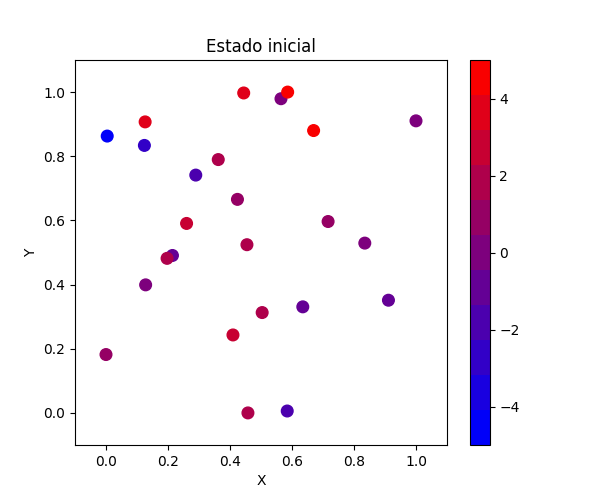
\includegraphics[width=\textwidth]{Images/Images_c/p9pc_t0.png}
     \end{subfigure}
     \begin{subfigure}[b]{0.3\textwidth}
         \centering
         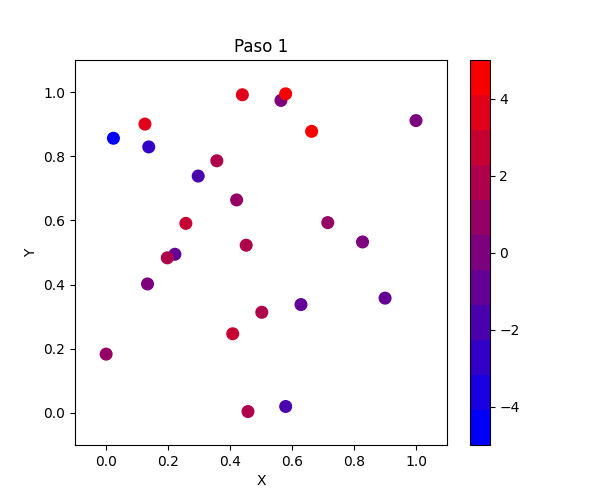
\includegraphics[width=\textwidth]{Images/Images_c/p9pc_t01.png}
     \end{subfigure}
     \begin{subfigure}[b]{0.3\textwidth}
         \centering
         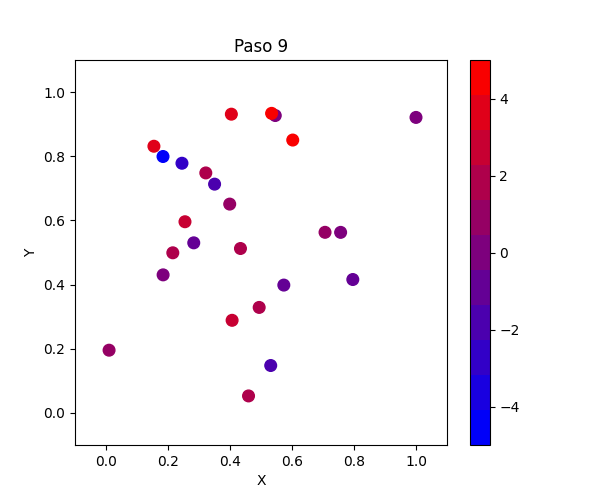
\includegraphics[width=\textwidth]{Images/Images_c/p9pc_t09.png}
     \end{subfigure}
     \begin{subfigure}[b]{0.3\textwidth}
         \centering
         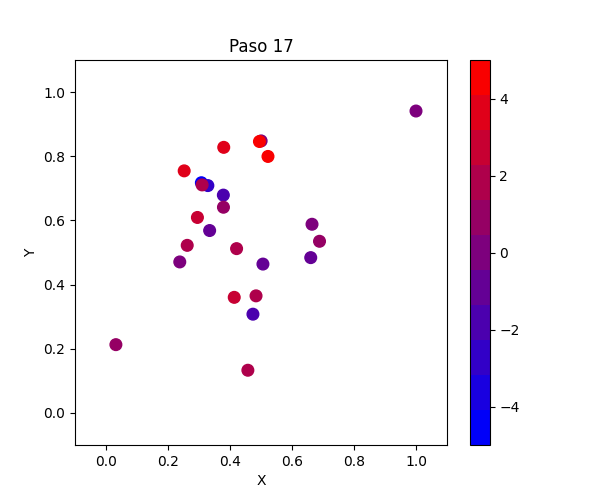
\includegraphics[width=\textwidth]{Images/Images_c/p9pc_t17.png}
     \end{subfigure}
     \begin{subfigure}[b]{0.3\textwidth}
         \centering
         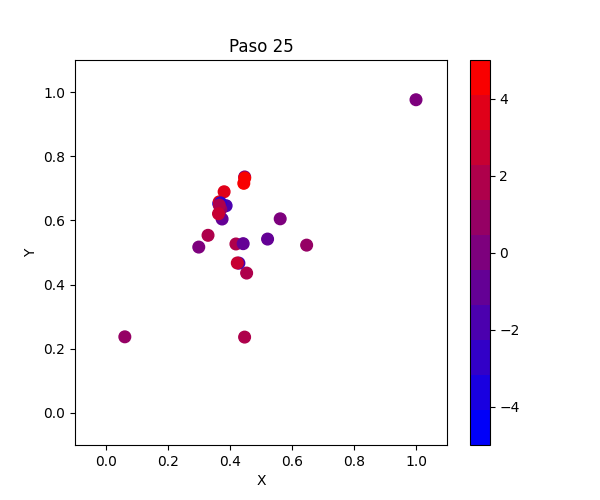
\includegraphics[width=\textwidth]{Images/Images_c/p9pc_t25.png}
     \end{subfigure}
     \begin{subfigure}[b]{0.3\textwidth}
         \centering
         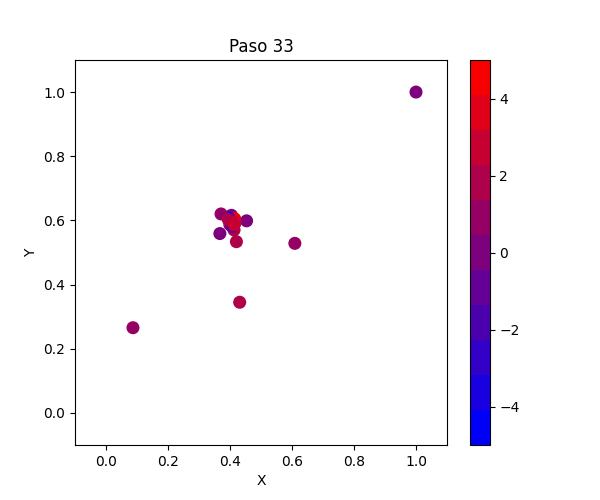
\includegraphics[width=\textwidth]{Images/Images_c/p9pc_t33.png}
     \end{subfigure}
          \begin{subfigure}[b]{0.3\textwidth}
         \centering
         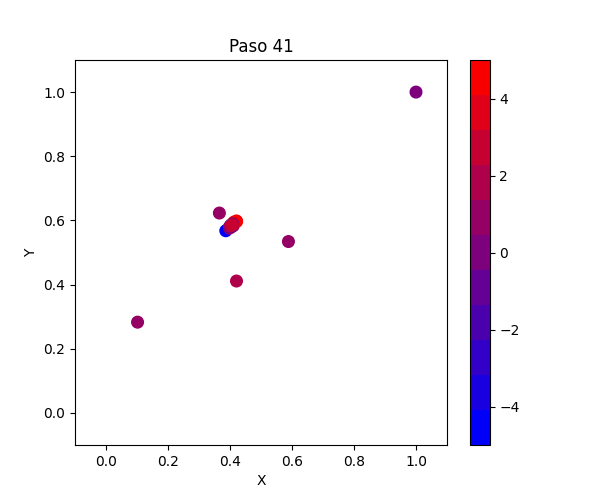
\includegraphics[width=\textwidth]{Images/Images_c/p9pc_t41.png}
     \end{subfigure}
     \begin{subfigure}[b]{0.3\textwidth}
         \centering
         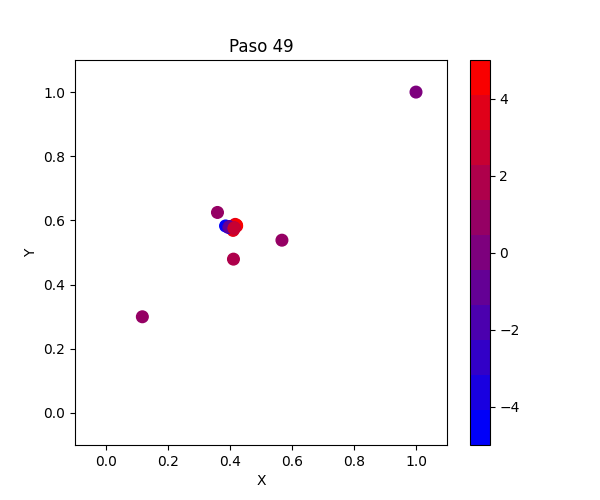
\includegraphics[width=\textwidth]{Images/Images_c/p9pc_t49.png}
     \end{subfigure}
     \begin{subfigure}[b]{0.3\textwidth}
         \centering
         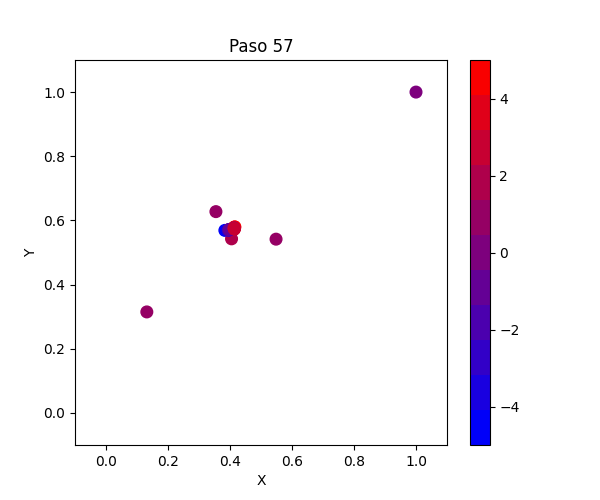
\includegraphics[width=\textwidth]{Images/Images_c/p9pc_t57.png}
     \end{subfigure}
     \caption{Movimiento de part\'iculas con carga.}
     \label{fig1}
\end{figure}

\newpage

La figura \ref{fig2} muestra el movimiento de las part\'iculas al actuar sobre ellas la fuerza de gravedad previamente establecida. En este caso, el tama\~no de la part\'icula es indicador de la cantidad de masa que tiene. Se puede observar que la convergencia ocurre a mayor velocidad que las part\'iculas con carga, lo cual puede indicar que, en este universo, la fuerza de gravedad es mayor que las de atracci\'on y repulsi\'on. Una \href{https://github.com/FeroxDeitas/Simulacion-Nano/blob/main/Tareas/P9/Images/images_m/movement_m.gif}{visualizaci\'on} animada del movimiento puede encontrarse en el repositorio en GitHub de J. Torres.

\begin{figure}[h]
\centering
     \begin{subfigure}[b]{0.3\textwidth}
         \centering
         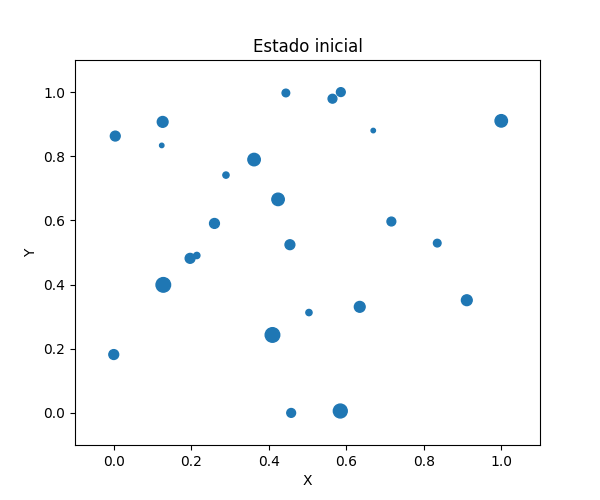
\includegraphics[width=\textwidth]{Images/Images_m/p9pm_t0.png}
     \end{subfigure}
     \begin{subfigure}[b]{0.3\textwidth}
         \centering
         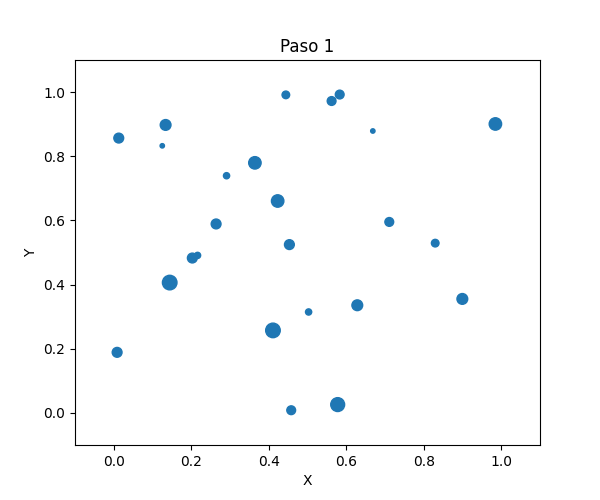
\includegraphics[width=\textwidth]{Images/Images_m/p9pm_t01.png}
     \end{subfigure}
     \begin{subfigure}[b]{0.3\textwidth}
         \centering
         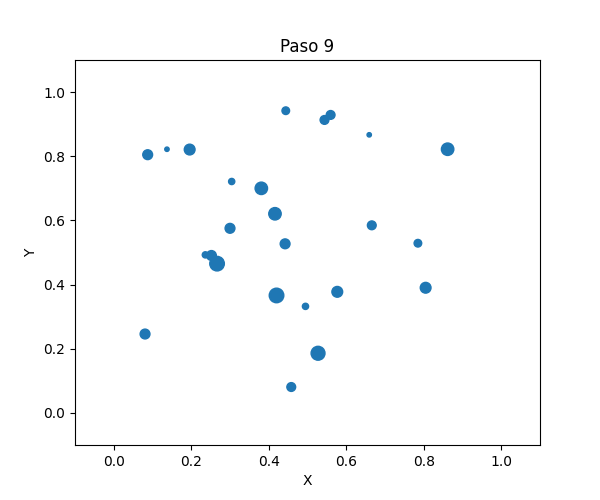
\includegraphics[width=\textwidth]{Images/Images_m/p9pm_t09.png}
     \end{subfigure}
     \begin{subfigure}[b]{0.3\textwidth}
         \centering
         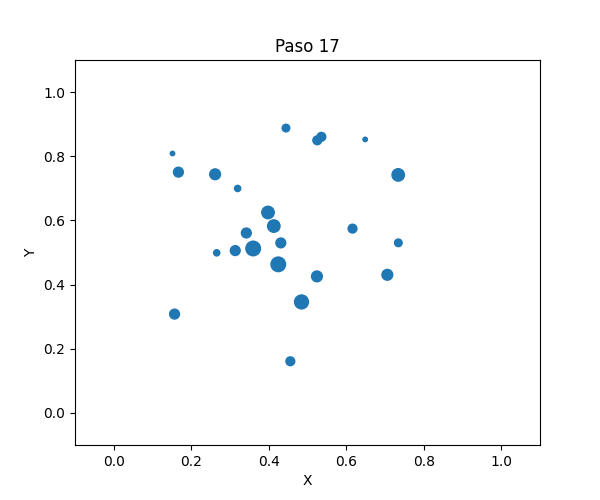
\includegraphics[width=\textwidth]{Images/Images_m/p9pm_t17.png}
     \end{subfigure}
     \begin{subfigure}[b]{0.3\textwidth}
         \centering
         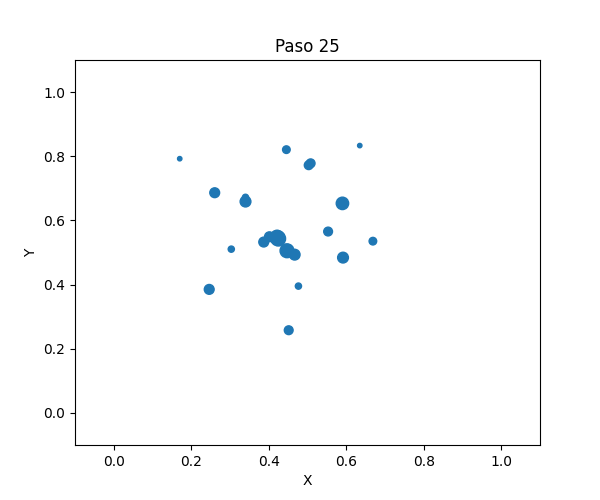
\includegraphics[width=\textwidth]{Images/Images_m/p9pm_t25.png}
     \end{subfigure}
     \begin{subfigure}[b]{0.3\textwidth}
         \centering
         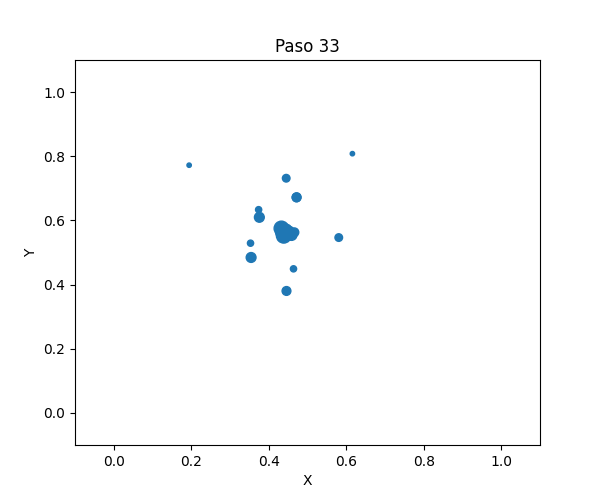
\includegraphics[width=\textwidth]{Images/Images_m/p9pm_t33.png}
     \end{subfigure}
          \begin{subfigure}[b]{0.3\textwidth}
         \centering
         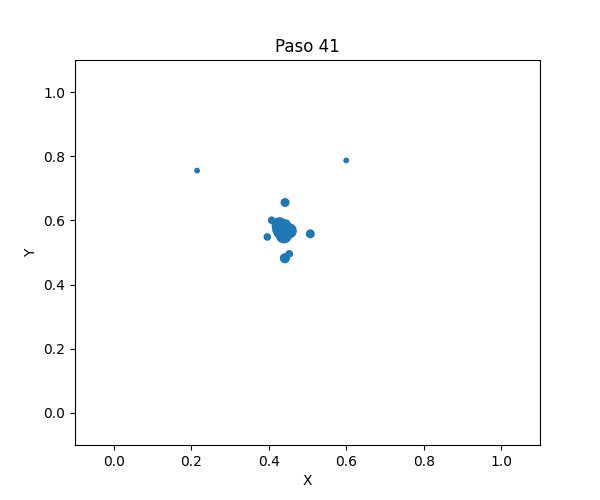
\includegraphics[width=\textwidth]{Images/Images_m/p9pm_t41.png}
     \end{subfigure}
     \begin{subfigure}[b]{0.3\textwidth}
         \centering
         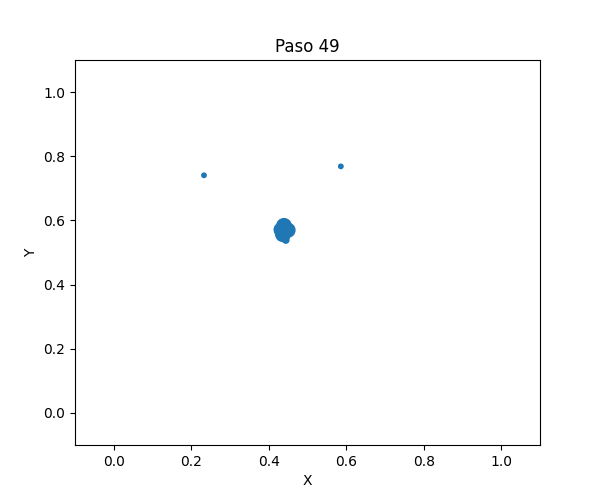
\includegraphics[width=\textwidth]{Images/Images_m/p9pm_t49.png}
     \end{subfigure}
     \begin{subfigure}[b]{0.3\textwidth}
         \centering
         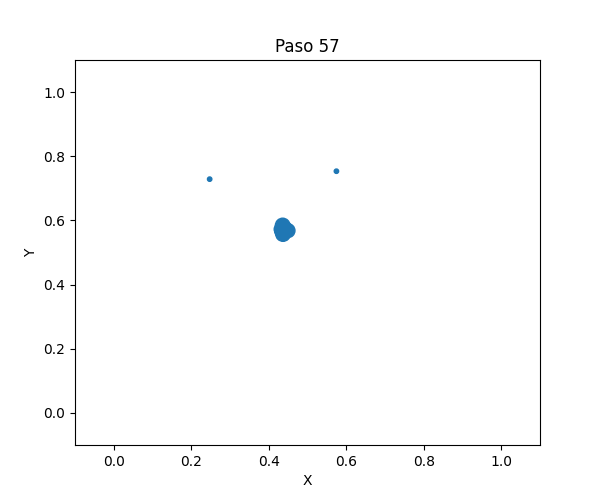
\includegraphics[width=\textwidth]{Images/Images_m/p9pm_t57.png}
     \end{subfigure}
     \caption{Movimiento de part\'iculas con masa.}
     \label{fig2}
\end{figure}

\newpage

En la figura \ref{fig3} se representa el movimiento de las part\'iculas cuando act\'uan sobre ellas las fuerzas de atracci\'on, repulsi\'on y de gravedad. Se observan velocidades un tanto mayores a ambos casos previos, por lo que las part\'iculas convergen antes. Esto es de esperarse, ya que existen dos fuerzas que act\'uan en favor de la atracci\'on de las part\'iculas. Una \href{https://github.com/FeroxDeitas/Simulacion-Nano/blob/main/Tareas/P9/Images/images_mc/movement_mc.gif}{visualizaci\'on} animada del experimento puede encontrarse en el repositorio en GitHub de J. Torres.

\begin{figure}[h]
\centering
     \begin{subfigure}[b]{0.3\textwidth}
         \centering
         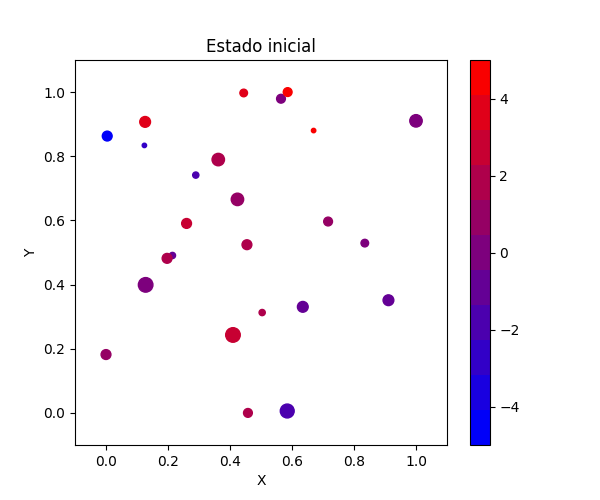
\includegraphics[width=\textwidth]{Images/Images_mc/p9pmc_t0.png}
     \end{subfigure}
     \begin{subfigure}[b]{0.3\textwidth}
         \centering
         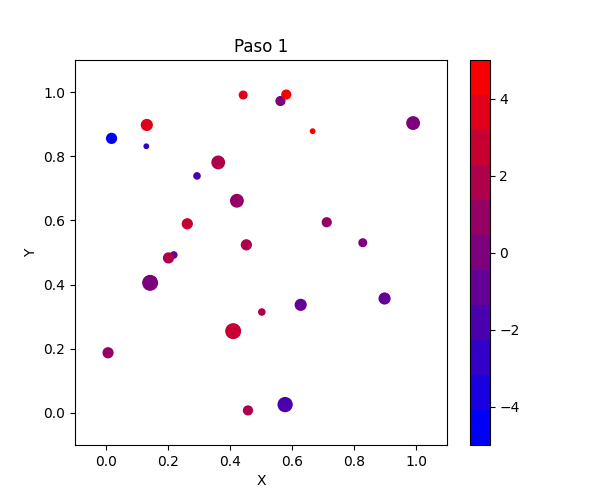
\includegraphics[width=\textwidth]{Images/Images_mc/p9pmc_t01.png}
     \end{subfigure}
     \begin{subfigure}[b]{0.3\textwidth}
         \centering
         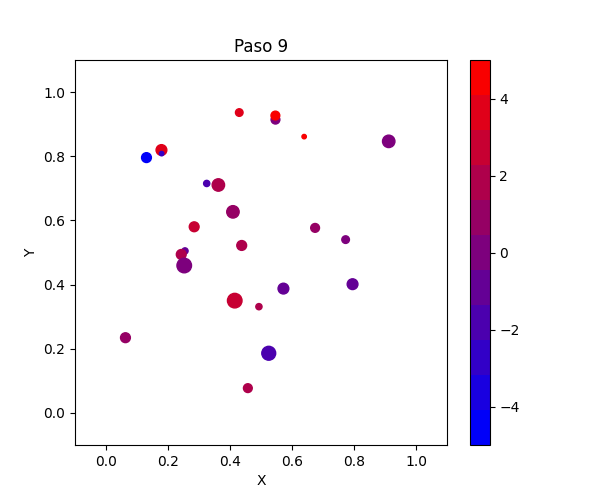
\includegraphics[width=\textwidth]{Images/Images_mc/p9pmc_t09.png}
     \end{subfigure}
     \begin{subfigure}[b]{0.3\textwidth}
         \centering
         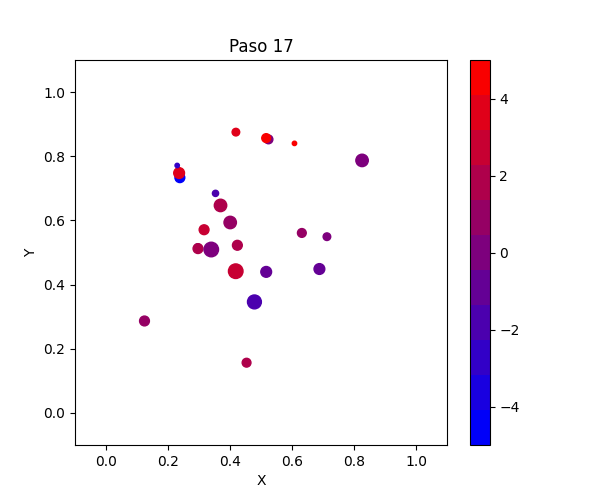
\includegraphics[width=\textwidth]{Images/Images_mc/p9pmc_t17.png}
     \end{subfigure}
     \begin{subfigure}[b]{0.3\textwidth}
         \centering
         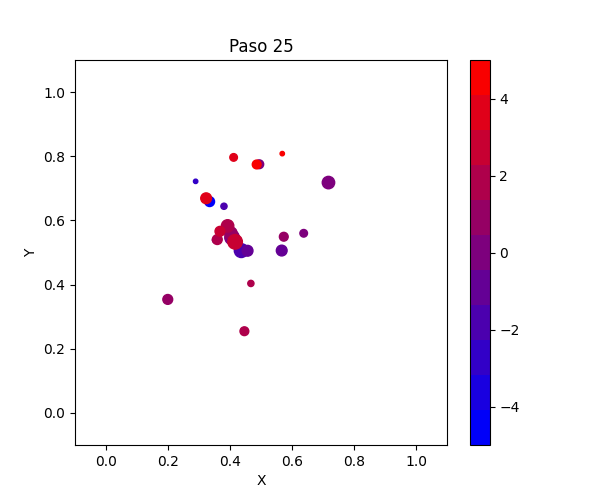
\includegraphics[width=\textwidth]{Images/Images_mc/p9pmc_t25.png}
     \end{subfigure}
     \begin{subfigure}[b]{0.3\textwidth}
         \centering
         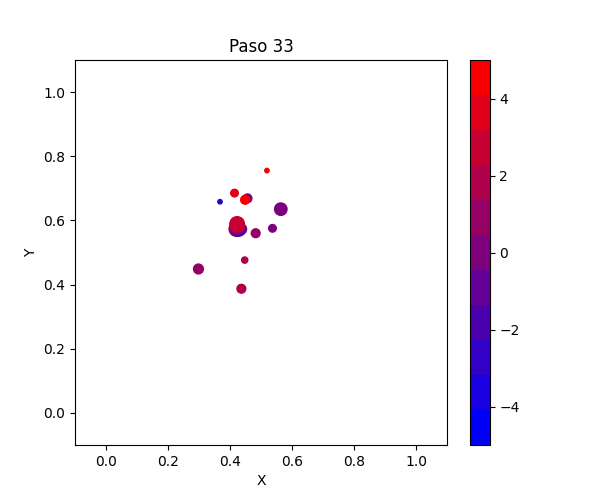
\includegraphics[width=\textwidth]{Images/Images_mc/p9pmc_t33.png}
     \end{subfigure}
          \begin{subfigure}[b]{0.3\textwidth}
         \centering
         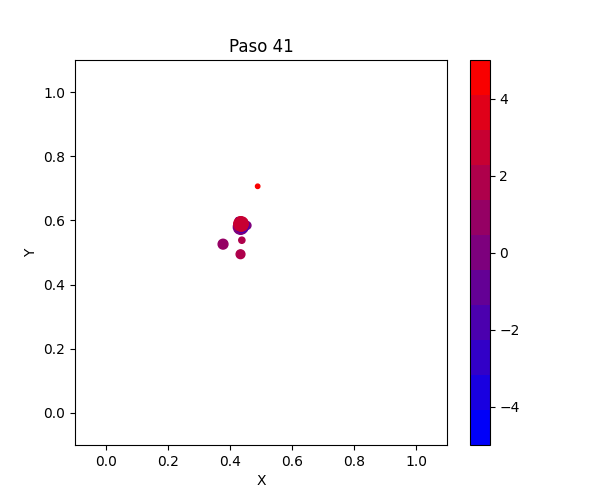
\includegraphics[width=\textwidth]{Images/Images_mc/p9pmc_t41.png}
     \end{subfigure}
     \begin{subfigure}[b]{0.3\textwidth}
         \centering
         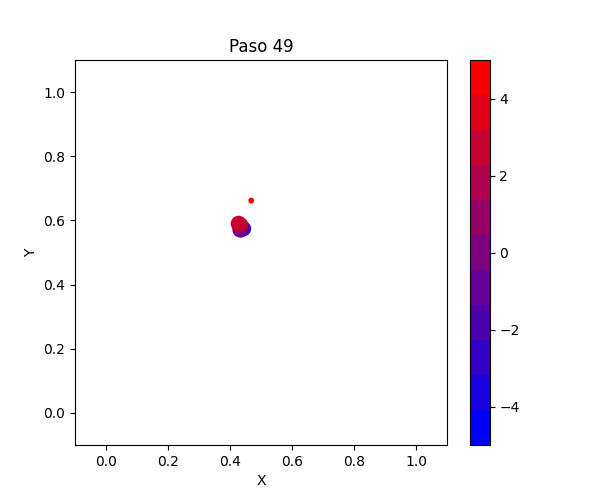
\includegraphics[width=\textwidth]{Images/Images_mc/p9pmc_t49.png}
     \end{subfigure}
     \begin{subfigure}[b]{0.3\textwidth}
         \centering
         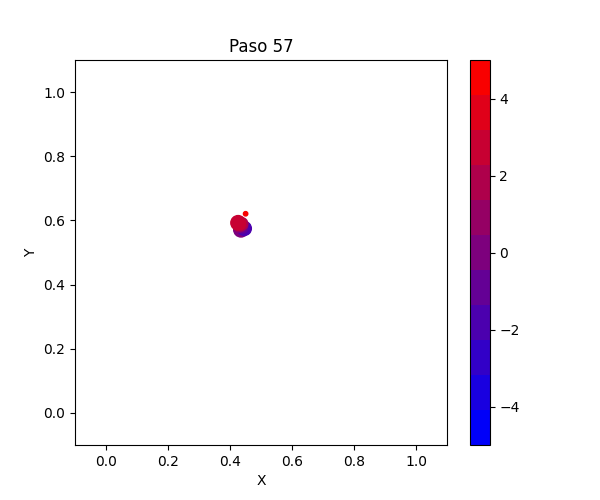
\includegraphics[width=\textwidth]{Images/Images_mc/p9pmc_t57.png}
     \end{subfigure}
     \caption{Movimiento de part\'iculas con carga y masa.}
     \label{fig3}
\end{figure}

\newpage

En la figura \ref{fig4} se pueden observar las distribuciones de las velocidades de cada part\'icula para cada iteraci\'on del experimento. En la figura \ref{fig:carga}, las part\'iculas se mueven debido a las fuerzas de atracci\'on y repulsi\'on, la figura \ref{fig:masa} muestra las velocidades de las part\'iculas al actuar sobre ellas la fuerza de gravedad y en la figura \ref{fig:mascar} las part\'iculas se mueven debido a la suma de fuerzas de atracci\'on, repulsi\'on y de gravedad.

\begin{figure}[h]
\centering
    \begin{subfigure}[b]{0.49\textwidth}
         \centering
         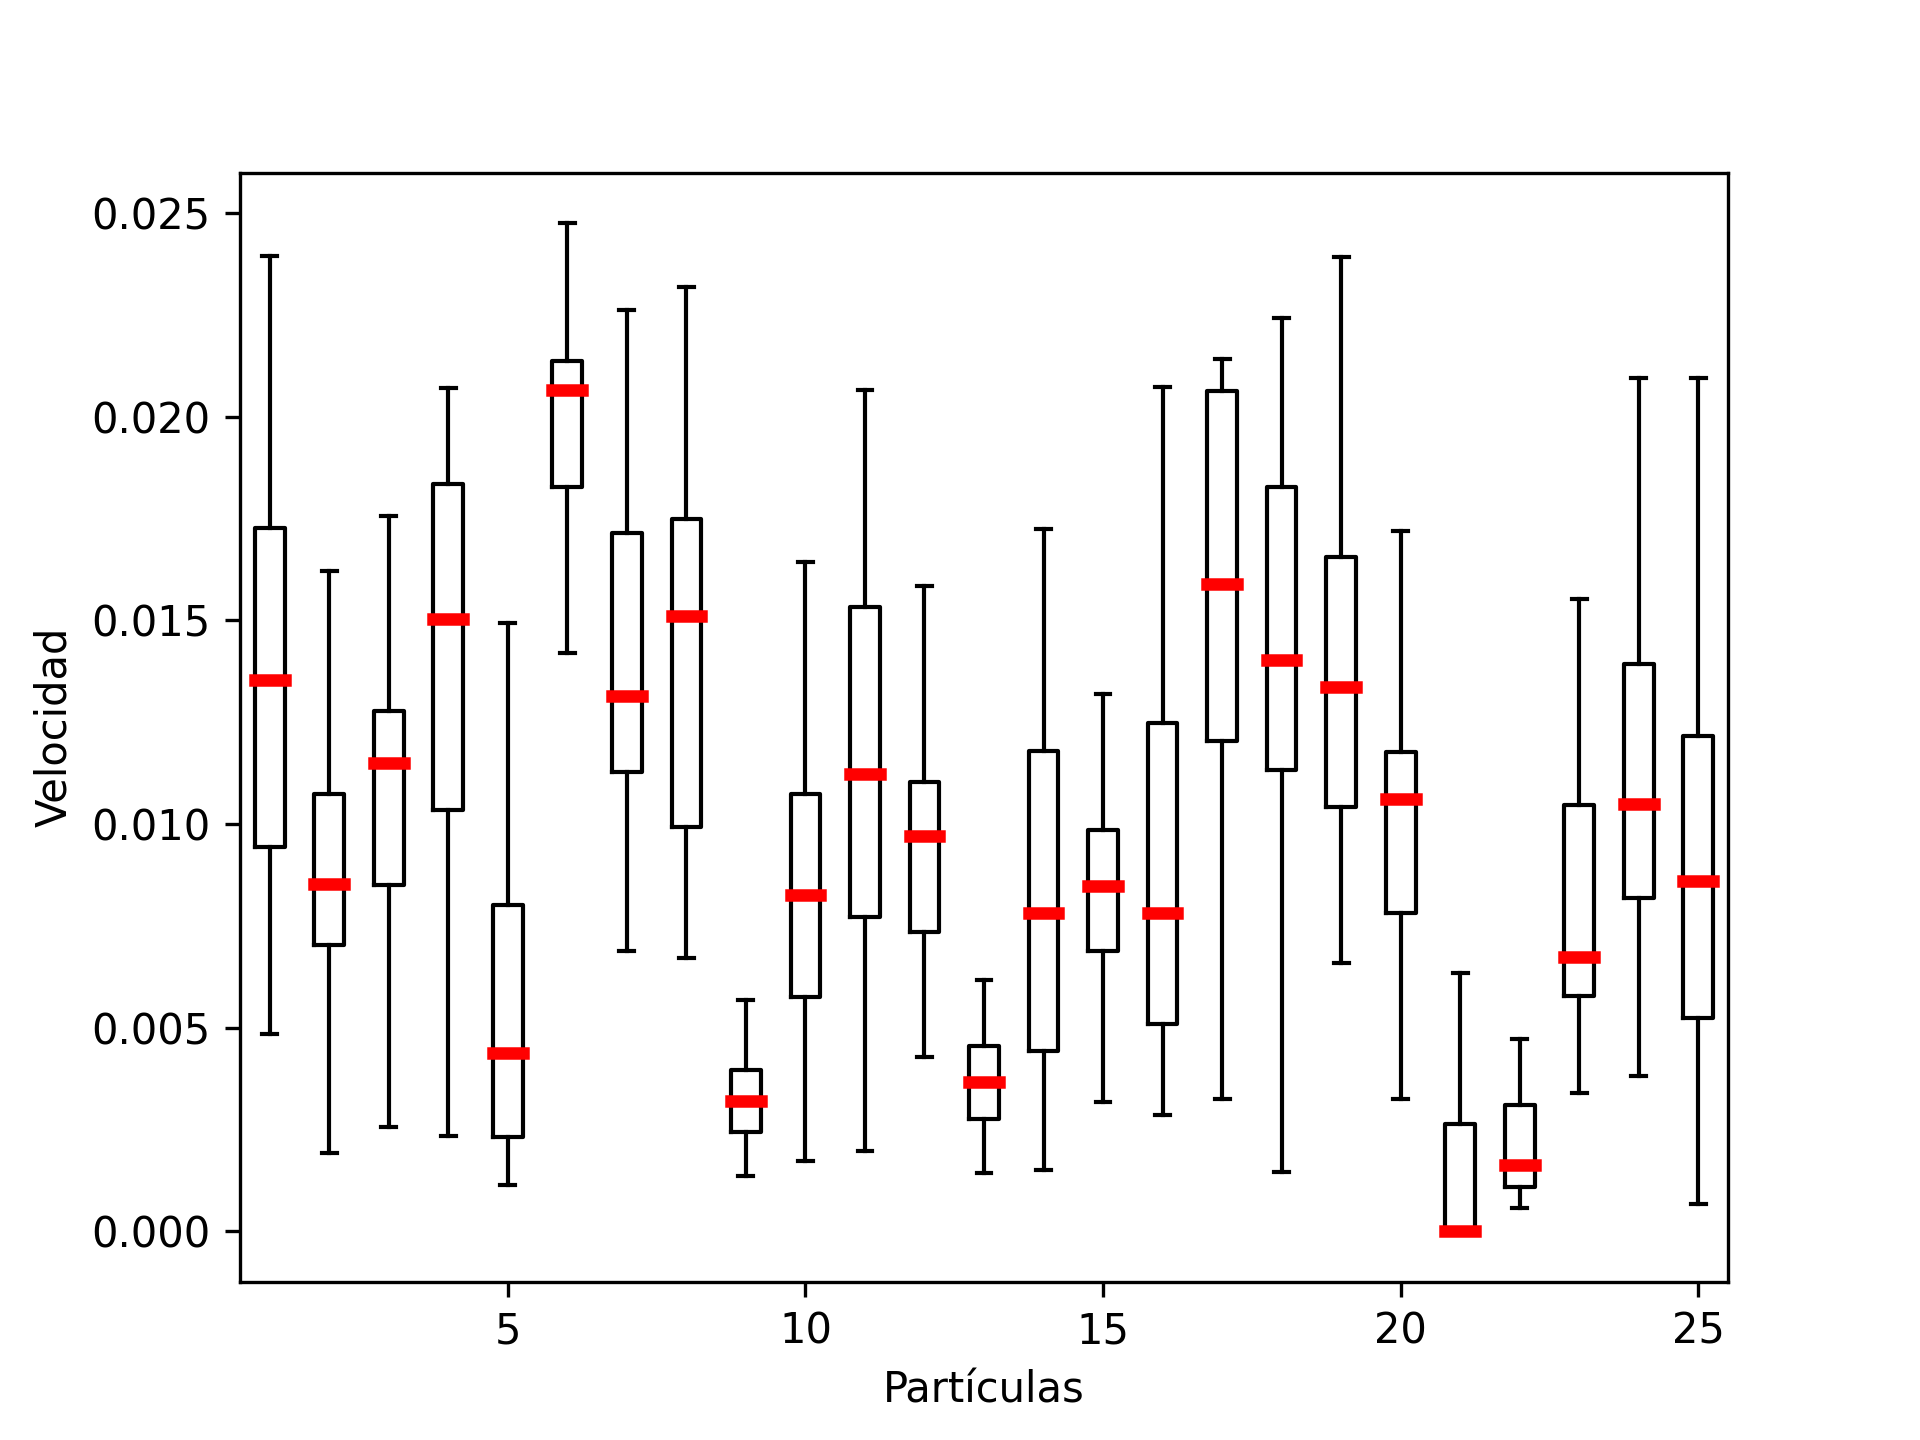
\includegraphics[width=\textwidth]{Images/p9pc.png}
         \caption{Velocidades de part\'iculas con carga.}
         \label{fig:carga}
    \end{subfigure}
    \begin{subfigure}[b]{0.49\textwidth}
         \centering
         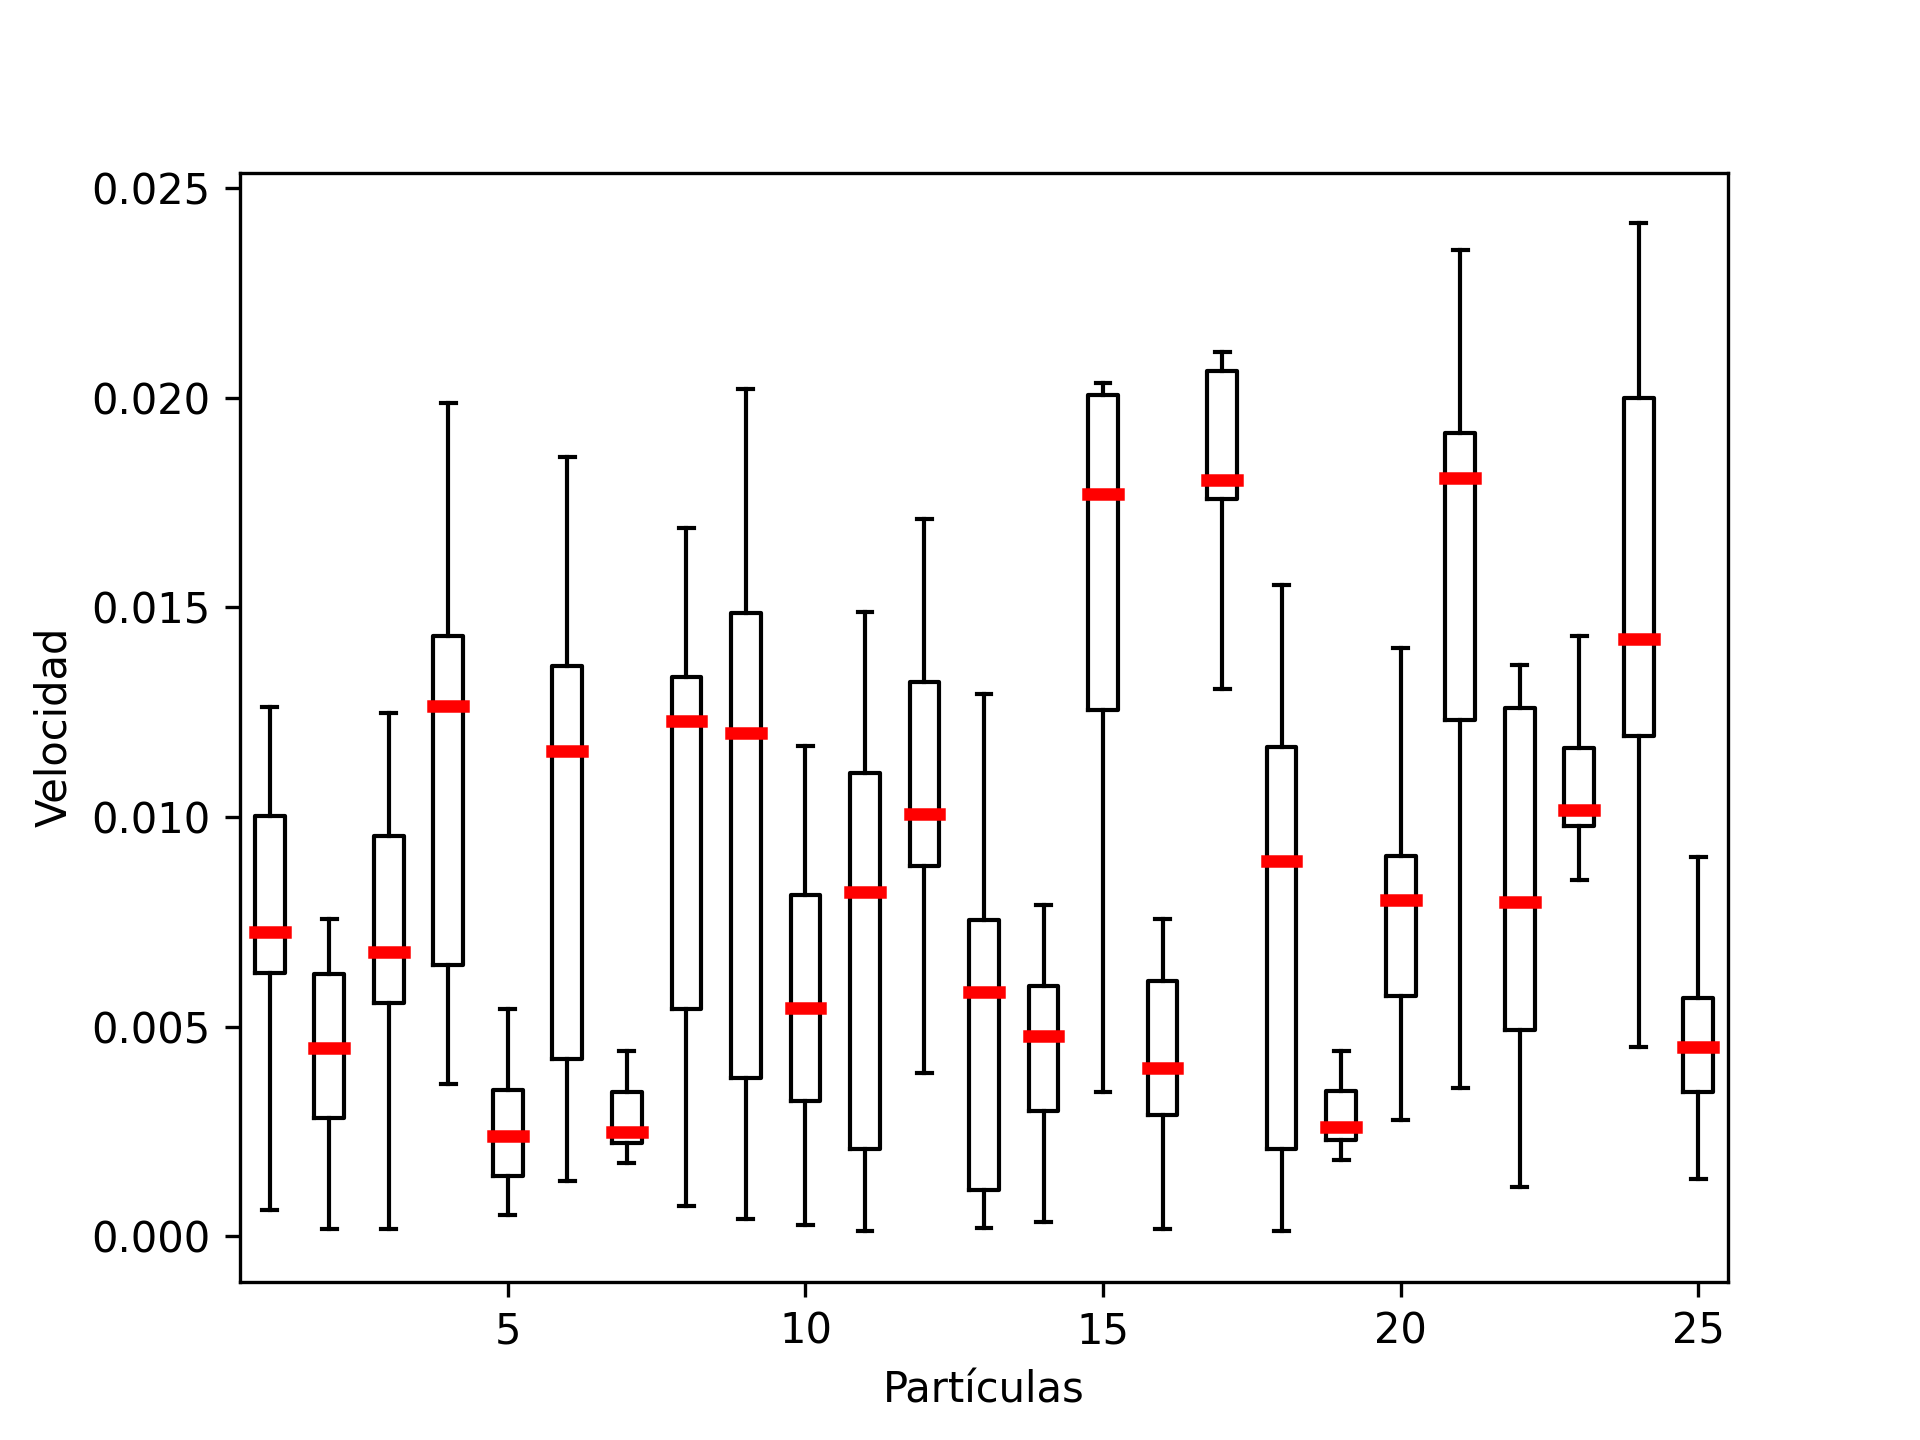
\includegraphics[width=\textwidth]{Images/p9pm.png}
         \caption{Velocidades de part\'iculas con masa.}
         \label{fig:masa}
    \end{subfigure}
    \begin{subfigure}[b]{0.49\textwidth}
         \centering
         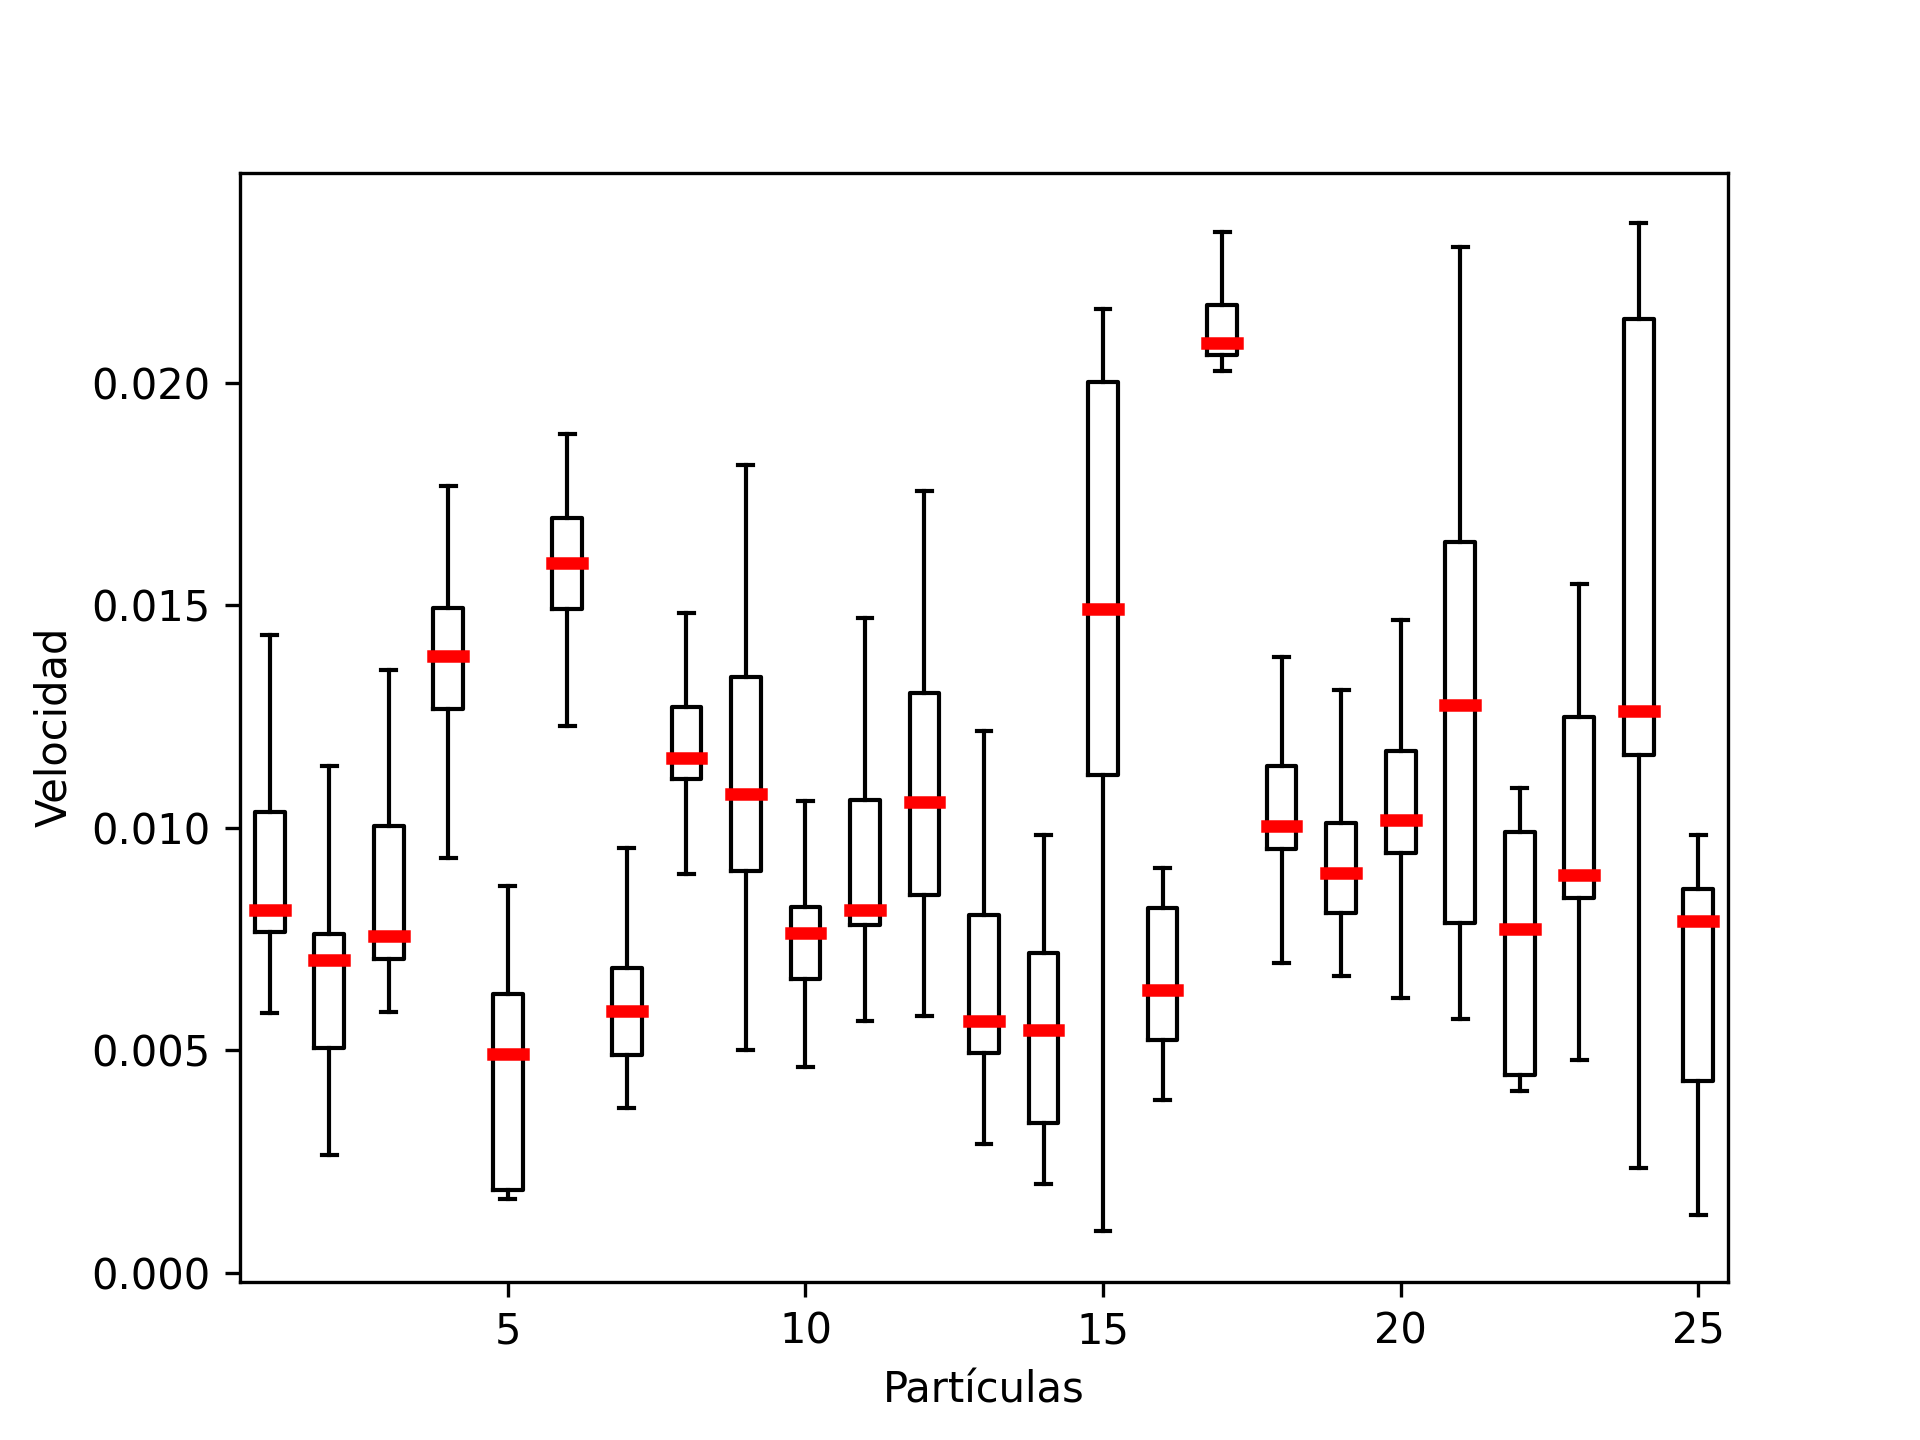
\includegraphics[width=\textwidth]{Images/p9pmc.png}
         \caption{Velocidades de part\'iculas con carga y masa.}
         \label{fig:mascar}
    \end{subfigure}
    \caption{Distribuci\'on de velocidades de las part\'iculas para cada tipo de experimento.}
    \label{fig4}
\end{figure}

Se ha realizado tambi\'en un an\'alisis estad\'istico de varianza tipo ANOVA para verificar si existe una diferencia significativa entre las velocidades de una part\'icula al estar sometida a los diferentes tipos de fuerza. El valor $p$ encontrado por el an\'alisis es mucho menor a 0.05, por lo que se puede concluir que la diferencia s\'i es estad\'isticamente significativa.

\newpage

\section{Conclusiones}

Observando las visualizaciones de los movimientos de las part\'iculas, se puede encontrar una diferencia notable en velocidades. Al observar las distribuciones en los diagramas caja-bigote, esta diferencia se puede apreciar m\'as claramente, habiendo un incremento considerable en velocidad al implementar ambas fuerzas en el movimiento. El an\'alisis de varianza confirma esta diferencia, por lo que se puede concluir que existe una relaci\'on entre la fuerza que se aplica y la velocidad de las part\'iculas.

\chapter{Reto 1}

\section{Objetivo}
El reto 1 consiste en desarrollar la simulaci\'on de dos diferentes tipos de objetos: bolitas duras grandes y partículas frágiles — cuando una partícula es atrapada entre dos bolas, se modifica: si está sola, se fragmenta, pero si hay otras partículas en ese mismo traslape de dos bolas, se pegan todos juntos.

\section{Desarrollo}
El desarrollo del reto est\'a basado en el \href{https://satuelisa.github.io/simulation/p9.html}{c\'odigo} descrito por E. Schaeffer para la pr\'actica 9 de su curso de simulaci\'on. En primer lugar, con el c\'odigo \ref{codigo11} se crean $m=7$ bolas y $n=25$ part\'iculas. Se les asignan posiciones $(x, y)$, y velocidades $(vx, vy)$, as\'i como un tama\~no $r$ iniciales. Estos valores se guardan en marcos de datos para su posterior uso en el c\'odigo.

\begin{lstlisting}[caption=Creaci\'on de Bolas y Part\'iculas, label=codigo11, language=Python]
m = 7
vx = (2 * (np.random.uniform(size = m) < 0.5) - 1) * np.random.uniform(low = 0.01, high = 0.04, size = m)
vy = (2 * (np.random.uniform(size = m) < 0.5) - 1) * np.random.uniform(low = 0.01, high = 0.04, size = m)
x = np.random.uniform(size = m)
y = np.random.uniform(size = m)
r = np.random.uniform(low = 0.05, high = 0.1, size = m)
bolas = pd.DataFrame({'x': x, 'y': y, 'dx': vx, 'dy': vy, 'r': r})
n = 50
vx = (2 * (np.random.uniform(size = n) < 0.5) - 1) * np.random.uniform(low = 0.02, high = 0.05, size = n)
vy = (2 * (np.random.uniform(size = n) < 0.5) - 1) * np.random.uniform(low = 0.02, high = 0.05, size = n)
x = np.random.uniform(size = n)
y = np.random.uniform(size = n)
print(x)
r = np.random.uniform(low = 0.01, high = 0.03, size = n)
particulas = pd.DataFrame({'x': x, 'y': y, 'dx': vx, 'dy': vy, 'r': r,\
                           'v': [1] * n, 'a': [1] * n})
\end{lstlisting}

Con el c\'odigo \ref{codigo12} se verifica que las part\'iculas est\'en en movimiento y, si lo est\'an, se calculan las distancias entre part\'iculas y bolas para saber si est\'an sobrelapadas.

\begin{lstlisting}[caption=Verificaci\'on de Sobrelapamiento de Part\'iculas y Bolas, label=codigo12, language=Python]
for t in range(25):
    
    for i in range(n):
        p = particulas.iloc[i]
        v = p.v
        
        if v > 0:
            pr = p.r
            px = p.x
            py = p.y
            conteo = 0
            for k in range(m):
                pk = bolas.iloc[k]
                pkr = pk.r
                pkx = pk.x
                pky = pk.y
                dx = px - pkx
                dy = py - pky
                dr = pkr + pr
                d = sqrt(dx**2 + dy**2)
                if d < dr:
                    conteo += 1
\end{lstlisting}

En el c\'odigo \ref{codigo13} se realiza la uni\'on de las part\'iculas cuando existen dos o m\'as de ellas sobrelapadas entre dos bolas.

\begin{lstlisting}[caption=Uni\'on de Part\'iculas Sobrelapadas, label=codigo13, language=Python]
            if conteo >= 2:
                conteo2 = 0
                for j in range(n):
                    if i != j:
                        pj = particulas.iloc[j]
                        pjr = pj.r
                        pjx = pj.x
                        pjy = pj.y
                        dx = px - pjx
                        dy = py - pjy
                        dr = pjr + pr
                        d = sqrt(dx**2 + dy**2)
                        if d < dr:
                            conteo2 += 1
                            a1 = np.pi * (pr**2)
                            a2 = np.pi * (pjr**2)
                            a = a1 + a2
                            rt = sqrt(a/np.pi)
                            particulas.at[i, 'r'] = rt
                            particulas.at[j, 'v'] = -1
\end{lstlisting}

Para fragmentar las part\'iculas  que se encuentren solas en un traslape de dos bolas, se implementa el c\'odigo \ref{codigo14}. Se actualizan las posiciones, velocidades y tama\~nos de las part\'iculas.

\begin{lstlisting}[caption=Fragmentaci\'on de Part\'iculas Sobrelapadas, label=codigo14, language=Python]
                if conteo2 == 0:
                    v = random()
                    v1 = 1 - v
                    vx1 = p.dx * -1
                    vy1 = p.dy * -1
                    a = np.pi * (pr**2)
                    a1 = a * v
                    a2 = a * v1
                    r1 = sqrt(a1/np.pi)
                    r2 = sqrt(a2/np.pi)
                    particulas.at[i, 'r'] = r1
                    particulas = particulas.append({'x': px, 'y': py, 'dx': vx1, 'dy': vy1,\
                                                    'r': r2, 'v': 1, 'a': 1}, ignore_index=True)
\end{lstlisting}

El c\'odigo \ref{codigo15} elimina las part\'iculas vac\'ias que quedan despu\'es del c\'alculo y hace un recuento de la cantidad de part\'iculas que quedan. Adem\'as, se guardan los datos de bolas y part\'iculas en archivos de tipo CSV para su posterior uso en la visualizaci\'on del movimiento.

\begin{lstlisting}[caption=Eliminacio\'on de Part\'iculas Vac\'ias y Guardado de Datos, label=codigo15, language=Python]
    particulas = particulas.loc[particulas['v'] > 0]
    n = particulas.shape[0]
    particulas.to_csv('p_part_{:d}.dat'.format(t), header = False, index = False)
    bolas.to_csv('p_bola_{:d}.dat'.format(t), header = False, index = False)
\end{lstlisting}

El c\'odigo \ref{codigo16} hace que las bolas reboten de los l\'imites del marco de coordenadas, mientras que el c\'odigo \ref{codigo17} hace lo mismo para las part\'iculas.\\

\begin{lstlisting}[caption=Rebote de las Bolas en los L\'imites, label=codigo16, language=Python]
    for i in range(m):
        b = bolas.iloc[i]
        br = b.r
        bx = b.x
        by = b.y
        vx = b.dx
        vy = b.dy
        x = bx + vx
        y = by + vy
        if 0 >= (x-br):
            x = 0 + br
            bolas.at[i, 'dx'] = vx * -1
        elif (x+br) >= 1:
            x = 1 - br
            bolas.at[i, 'dx'] = vx * -1
        if 0 >= (y-br):
            y = 0 + br
            bolas.at[i, 'dy'] = vy * -1
        elif (y+br) >= 1:
            y = 1 - br
            bolas.at[i, 'dy'] = vy * -1
        
        bolas.at[i, 'x'] = x
        bolas.at[i, 'y'] = y
\end{lstlisting}

\begin{lstlisting}[caption=Rebote de las Part\'iculas en los L\'imites, label=codigo17, language=Python]
    for i in range(n):
        b = particulas.iloc[i]
        br = b.r
        bx = b.x
        by = b.y
        vx = b.dx
        vy = b.dy
        x = bx + vx
        y = by + vy
        if 0 >= (x-br):
            x = 0 + br
            particulas.at[i, 'dx'] = vx * -1
        elif (x+br) >= 1:
            x = 1 - br
            particulas.at[i, 'dx'] = vx * -1
        if 0 >= (y-br):
            y = 0 + br
            particulas.at[i, 'dy'] = vy * -1
        elif (y+br) >= 1:
            y = 1 - br
            particulas.at[i, 'dy'] = vy * -1
        
        particulas.at[i, 'x'] = x
        particulas.at[i, 'y'] = y
\end{lstlisting}

\section{Resultados}
Los movimientos de las bolas y part\'iculas, as\'i como la uni\'on y fragmentaci\'on de las part\'iculas se muestran en una \href{https://github.com/FeroxDeitas/Simulacion-Nano/blob/main/Tareas/P9/Images/p9pr.gif}{animaci\'on} de formato GIF contenida en el repositorio en GitHub de J. Torres, y realizada por medio de Gnuplot con los datos obtenidos del c\'odigo \ref{codigo15}, introduciendo el c\'odigo \ref{codigo18}.

\begin{lstlisting}[caption=Animaci\'on por Medio de Gnuplot, label=codigo18, language=Gnuplot]
set term gif animate delay 50
set key off
set datafile separator ","
set size square
set xrange [ -0.02 : 1.02] noreverse nowriteback
set yrange [ -0.02 : 1.02 ] noreverse nowriteback
set output 'p9pr.gif'
do for [i=0:24] {
  set title 'Paso '.(i + 1)
  plot 'p_bola_'.i.'.dat' u 1:2:5 w circles lc rgb "blue" fs solid noborder, \
       'p_part_'.i.'.dat' u 1:2:5 w circles lc rgb "red" fs solid noborder
}
\end{lstlisting}

\section{Conclusiones}
Por medio de este modelo se puede apreciar la simulaci\'on de uni\'on y fragmentaci\'on de part\'iculas al estar presente un agente que facilite la interacci\'on entre ellas. En cierto modo, es parecido al comportamiento que tendr\'ian las nanopart\'iculas de alg\'un material al estar en presencia de un agente catalizador o de otras nanopart\'iculas. Sin embargo, el comportamiento es demasiado simple como para describir en su totalidad un sistema de ese tipo, por lo que se necesitar\'ian realizar modificaciones si se requiere una simulaci\'on m\'as realista.

\bibliography{tarea_9}
\bibliographystyle{plainnat}

\end{document}
